\documentclass{ifda}
\usepackage{graphicx}
\graphicspath{ {./images/} }

%AUTHOR: the preferred method to generate PDF output is to use 'pdflatex'
%To clean up after a successful build, try: 'latexmk -c main.tex'


%EDITOR: replace X's to set the data for the header and footer
\newcommand{\thefirstpagenum}[0]{1}
%Year written
\newcommand{\theyear}[0]{2021}
\newcommand{\thevol}[0]{X}
%DOI if applicable
%\newcommand{\thedoi}[0]{enter DOI here}
\newcommand{\ledgerpages}[0]{\thefirstpagenum-\thelastpagenum}


%AUTHOR: please set these to generate correct PDF metadata
\hypersetup{pdfauthor={First Last}, pdftitle={This is a Title}}


%EDITOR: set the correct pageination during layout
\setcounter{page}{\thefirstpagenum}


%AUTHOR: this can be used to highlight changed text, surround with \edit{} and
%uncomment either to determine color
%\newcommand{\edit}[1]{{\color{red} #1}}
\newcommand{\edit}[1]{#1}

\overfullrule=10pt

%title here
\title{\\[1cm] Siege, a physics-based game for FPGA\newline Game report}
%Author info here
\author{Felix Bowyer}

\pagestyle{pagemain}


%The Author should select the appropriate pretitle below:
\pretitle{
  \centering \selectfont \par
  %\includegraphics[scale=0.5]{images/logo_black.png}
  %\centering \selectfont REVIEW ARTICLE \par
  %\centering \selectfont RESEARCH ARTICLE \par 
  \fontsize{24pt}{28pt}\selectfont} % Title is centered and at 24pt


\begin{document}

\maketitle

\thispagestyle{pagefirst}

\tableofcontents

\newpage

%%%%%%%%%%%%%%%%%%%%%%%%%%%%%%%%%%%%%%%%%%%%

%define the following sections to hide their Section Number (Notes Style)
\ledgernotes

\section{Initial task}

\section{VGA Protocol}
\subsection{Overview}
The VGA protocol controls a screen with 5 outputs - 3 4-bit lines for red, green and blue pixel density, and 2 1-bit pulse control signals for horizontal and vertical sync.\\

VGA was created for CRT (Cathode ray tube) screens, which work by directing a single cathode ray across the screen, left to right, top to bottom. The intensity of the ray at a point determines the colour of the pixel at that point. Since a beam cannot be instantaneously moved, at the borders of the screen there are some "blanking" cycles in which no pixels are drawn, but the beam is given time to move across the screen to where the next pixel needs to be drawn.\\

\begin{figure}[h]
    \centering
    \includegraphics[width=0.6\textwidth]{ VESA_TimingDiagram.jpg }
    \caption{VGA blanking, border and display regions.}
    \label{fig:vga_sync}
\end{figure}

hsync and vsync are put high when the beam should be at the start of their respective blanking intervals. These sync signals tell the screen how to move the beam in order to produce the required resolution. There is also a small border region around the actual displayed area - this is mostly to prevent pixels being written during the blanking region. Although most screens are now LCD and therefore do no require a blanking interval, the VGA protocol is still the same regardless.\\

\subsection{Sync circuit design}
To prevent screen tearing, any processing which effects pixels shown on the screen should be done only in the blanking region. This stops the image being updated during drawing, preventing tearing.\\

For the game, hsync and vsync are controlled by two counters, \verb|hcount_reg| and \\\verb|vcount_reg|. \verb|hcount_reg| is incremented every clock cycle, and reset to 0 at the end of a row of pixels (at \verb|hcount_reg == 11'd1903|). \verb|vcount_reg| is incremented at the end of each row of pixels, and reset at the end of the last row (where \verb|vcount_reg == 10'd931|).\\

\begin{figure}[h]
    \centering
    \includegraphics[width=1\textwidth]{ sync }
    \caption{Code assigning hsync, vsync, and in\_drawing\_region.}
    \label{fig:sync_assignment}
\end{figure}

Not counting the blanking and border regions, we have a drawing region between virtual pixel 384 and 1823 horizontally, and 31 and 930 vertically. Therefore, the game has an addressable resolution of 1440x900.\\

The counter-controlled sync system is designed with the counters as D-type flip-flop counters, where hcount is enabled with the clock, and vcount is enabled once hcount reaches 1903 (at which point TC goes high). Comparators are used to assign a boolean value to hsync, vsync and in\_drawing\_region, based on the value of the counters.\\

\begin{figure}[h]
    \centering
    \begin{minipage}{0.55\textwidth}
        \centering
        \includegraphics[width=1\textwidth]{ circuit_sync }
        \caption{Design of counter-sync system.}
        \label{fig:sync_count}
    \end{minipage}\hfill
    \begin{minipage}{0.35\textwidth}
        \centering
        \includegraphics[width=1\textwidth]{ code1 }
        \caption{Verilog counter system.}
        \label{fig:code1}
    \end{minipage}
\end{figure}

In Verilog, this logic is implemented using an always statement, as seen in Fig. 4. Each count is a register which is incremented as described above. An assign statement is used with comparators in Fig. 2 to implement the rest of the logic. When this program is synthesised and implemented on the FPGA board, the resulting circuit is optimised to be very similar to the design in Fig. 3.\\

\subsection{Drawing a pixel}
In order to actually draw a pixel to the screen, we introduce the 12-bit \verb|pix| register (where \verb|pix[11:8]| is the 4 bits for red, \verb|pix[7:4]| is for green and \verb|pix[3:0]| is for blue). As module output, we have \verb|pix_{r,g,b}|, each of which is 4-bits and corresponds to the relevant pins of the VGA connector in the constraints file. hsync and vsync also directly correspond to a VGA pin in the contraints.\\

To choose the colour of a pixel to draw, we set pix to the desired 12-bit value. For example, to set it to a pure red, we could use \verb|pix <= 12'hF00|. When drawing, hcount and vcount are effectively used as pointers to the coordinates of the pixel to be drawn this clock cycle. Therefore, we can define a region (using comparators) in which we should draw a colour. For example, \verb|assign in_banner_region = ((hcount >= 384) && (hcount < 1824) &&|\\ \verb|(vcount >= 31) && (vcount < 131));|\footnote{Note that hcount and vcount values are offset to account for blanking and border regions.} defines the rectangular region in which to draw the info bar at the top of the screen (which is a sprite and will be explained in more detail later - for now assume it is a solid colour). If we want to draw coloured pixels in that region, we assign \verb|pix_{r,g,b}| to be coloured when hcount and vcount are in in the region, and black if not. Since 1 pixel is drawn per clock cycle in the drawing region, this doesn't use up any clock cycles unnecessarily to draw black outside the region.\\

\begin{figure}[h]
    \centering
    \includegraphics[width=0.5\textwidth]{ code2 }
    \caption{pix\{r,g,b\} assignment.}
    \label{fig:sync_assignment}
\end{figure}

Using this system, it becomes easy to define regions and colours to draw in those regions. However, to draw more complex images containing many colours, as well as transparency, we need to use sprites. 

\section{Sprites}
In Siege, sprites are stored in Block RAM (BRAM), which is implemented through Xilinx IP. Each sprite has a corresponding BRAM IP, which is created using a \verb|.coe| file, which contains 1 hexadecimal digit for each pixel in the sprite. This allows for a maximum of 16 colours per image. Although this number is low, the available BRAM on the FPGA board quite low, and so it is nessecary to decrease file sizes where possible.\\

To allow for a greater colour depth than the 4 bits of a hex digit, the game uses colour palettes. Each hex digit in a \verb|.coe| file corresponds to a 12-bit (3-hex digit, 1 per colour channel) code in the sprite's \verb|.mem| palette file. When sprites are drawn, the code in the \verb|.coe| file is used as an index to look up the higher-depth colour to draw. This allows the sprite \verb|.coe| files to be 3x smaller whilst retaining high colour depth. For most images, 16 colours is more than enough, and if more are required then most of the time the sprite can be split into separate sprites.\\

\subsection{Sprite file format}
A sprite's coe file consists of two things. Firstly, a \verb|memory_|\\ \verb|initialization_radix|, which tells Vivado which base the data in the file is. Since we are using 1 hex character per colour, this was set to \verb|16| for all files. Secondly, there is a \verb|memory_initialization_vector|, which contains the actual sprite, in the form of a list of hex characters.\newpage

\begin{figure}[h!]
    \centering
    \begin{minipage}{0.48\textwidth}
        \centering
        \includegraphics[width=1\textwidth]{ corner }
        \caption{A sprite .coe file.}
        \label{fig:sync_count}
    \end{minipage}\hfill
    \begin{minipage}{0.38\textwidth}
        \centering
        \includegraphics[width=1\textwidth]{ target }
        \caption{With the correct spacing, you can see the image zoomed out.}
        \label{fig:code1}
    \end{minipage}
\end{figure}

For every coe file, there is a corresponding palette \verb|.mem| file. This consists of a list of up to 16 12-bit hex-formatted colour codes (one for each hex digit in the coe file). When drawing the sprite, the hex digit in the coe file is used as an index to look up the correct colour code for the pixel.\\

\begin{figure}[h]
    \centering
    \includegraphics[width=0.7\textwidth]{ targetpalette }
    \caption{A palette mem file.}
    \label{fig:sync_assignment}
\end{figure}

\subsection{Generating sprites}
A Python script, \verb|image_quantizer_coe.py|, was created from scratch using Python's PIL library to generate coe and palette mem files. A copy is included in the appendix.\\

It works by first importing the pixels of an image and adjusting the colour depth to have maximum 16 colours in the image. It then searches through the resulting image, making a list of all colours present. Whilst going through all the pixels, the script assembles the coe file based on the colour it finds. Finally, the program assembles the palette file from the list of colours. Using these files, we can create a ROM IP block holding the coe file, and draw the sprite by decoding each hex value with the palette.\\

\subsection{Drawing the info bar}
The info bar is a sprite drawn at the top of the screen. In order to draw this sprite, we must set up a few things, starting with instantiating the IP block.\\

\subsubsection{ROM IP block}
ROM IP works by taking an address wire \verb|addra|. The data at this address is then output on a wire \verb|douta|. In this case, each input memory address corresponds to a 4-bit pixel value as imported from the coe file - once the ROM is clocked, this value is output on \verb|douta|. In order to run the VGA output, we earlier used a clock, which we can use for our ROM IP.\\

\begin{figure}[h]
    \centering
    
\includegraphics[width=0.6\textwidth]{ banner }
    \caption{The info bar's IP instantiation.}
    \label{fig:sync_assignment}
\end{figure}

\subsubsection{Selecting a pixel to draw}
So far, we have a wire \verb|banner_out|, which contains the pixel value, and \verb|banner_px_count|, containing the index of the pixel to lookup in block memory. Therefore, to access each pixel, we must increment \verb|banner_px_count| by 1 after drawing a pixel, allowing us to draw successive pixels in the order they are in memory.\\

We only want to draw pixels for a sprite in a certain area. To achieve this, we assign a boolean value representing rectangular region for the sprite to be drawn in, similarly to how \verb|in_drawing_region| was defined. When the program is drawing a pixel in this region, \verb|banner_px_count| should be incremented. This count is reset at the end of drawing each frame so that the 1st pixel is drawn first each time.\\

\begin{figure}[h]
    \centering
    \includegraphics[width=0.9\textwidth]{ increment }
    \caption{Defining the info banner region, and incrementing the pixel count.}
    \label{fig:sync_assignment}
\end{figure}

\subsubsection{Decoding a pixel value}
To draw the correct colour, we must use the value from the ROM's output to look up the colour in the palette. To achieve this, the palette mem file is imported into a 2d register using \verb|$readmemh|. Then, the output from the block memory \verb|banner_px_count| is used as an index into the palette array to obtain the colour of the pixel to draw. This actual colour code to be drawn is then stored in the \verb|pix| 12-bit register. As described in §2, the value in the pix register is assigned to the outputs \verb|pix_{r,g,b}|, in order to draw that colour to the screen.\\

\begin{figure}[h]
    \centering
    \includegraphics[width=0.6\textwidth]{ inreg }
    \caption{Decoding a pixel value with the palette, and assigning it to outputs.}
    \label{fig:sync_assignment}
\end{figure}

This system of using a pixel counter, which is incremented after a pixel from the sprite is drawn, changing the colour of the next pixel to draw is very successful in drawing sprites, and even allows multiple sprites to be drawn on top of each other.\\

\subsection{Drawing other sprites} %transparency
The info bar is in many ways an ideal sprite to draw - it has a fixed position, is a perfect rectangle, and doesn't require other sprites to be drawn on top of it. However, in the game, there are sprites which aren't so ideal - how do we draw them?\\

\subsubsection{Non-fixed position sprites}
The cannonball is a user-controlled moving sprite, which is shot across the screen. Therefore, it's position needs to be able to change.\\
The easiest way to do this under the current system is to assign the sprite's drawing region to be dependent on registers holding the current position of the cannonball. We assign the region as follows:\\
\verb|assign in_cannonball_region = ((hcount >= (384 + cannonball_x)) &&|\\ \verb|(hcount < (384 + cannonball_x + cannonball_size)) && (vcount >= (31 +|\\ \verb|cannonball_y)) && (vcount < (31 + cannonball_y + cannonball_size)));|\\

This causes the region that the cannonball is rendered in to vary with \verb|cannonball_x| and \verb|cannonball_y|, since \verb|in_cannonball_region| is just a combinatorial output wire of it's products.\\

\subsubsection{Non-rectangular sprites}
Not all sprites in the game are rectangular. In particular, the cannonball and target sprites are rough circles. Since for both sprites we need to be able to draw behind them, it is necessary to have transparency.\\

To achieve this, a sprite's palette is edited so that the background colour is \verb|001|. For example, if the image used to generate the script has an \verb|FFF| white background, then the palette can be manually edited to change \verb|FFF| to \verb|001|. Then, in order to make the background pixels render as transparent, there is a check on assigning \verb|pix|.\\
Checking the value of \verb|target_palette[target_out]| i.e. the colour of the pixel to render, and only assigning pix if it isn't 001, stops transparent areas from affecting the value of pix, allowing objects behind it to also render correctly.\\

\begin{figure}[h]
    \centering
    \includegraphics[width=0.7\textwidth]{ tgt2 }
    \caption{Checking for transparent pixels.}
    \label{fig:sync_assignment}
\end{figure}

\subsubsection{Changing sprites} %timer
The timer sprite shows the time passed in the game by increasing in size over time. Similarly to transparency, this is achieved by a check on the assignment. We use \verb|if (in_timer_region && (hcount < (394 + game_time + 1)) ) begin| as a condition (game\_time slowly increases). This is a quick way to stop any section past a certain point (394 + game\_time+ 1) from rendering. The power bar works in a similar way.\\

\subsubsection{Drawing priority}
Some sprites need to be drawn on top of others when drawing within the region of multiple sprites. The order of rendering is resolved by making several assignments to \verb|pix|, of which only the last is still stored in pix when \verb|pix_{r,g,b}| are assigned.\\

\section{Game design}

\subsection{Menus}
There is a start menu when the game is first started, and an end screen when the game is done. Each one has a sprite directing the player what to do to start the game. During the menu, no other sprites are shown.\\

\begin{figure}[h!]
    \centering
    \begin{minipage}{0.45\textwidth}
        \centering
        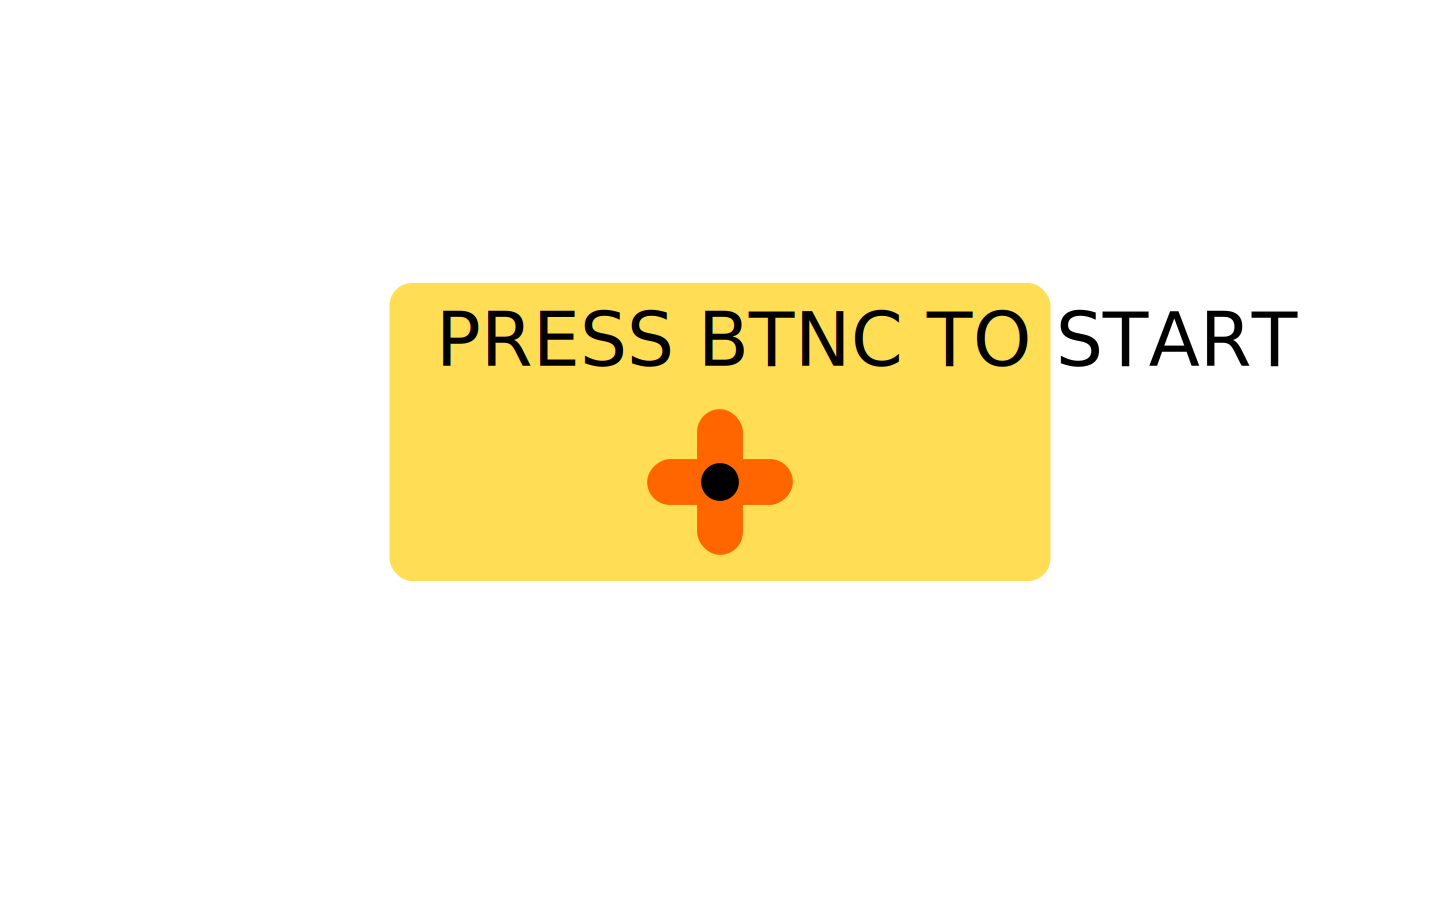
\includegraphics[width=1\textwidth]{ start }
        \caption{The start screen.}
        \label{fig:sync_count}
    \end{minipage}\hfill
    \begin{minipage}{0.40\textwidth}
        \centering
        \includegraphics[width=1\textwidth]{ end }
        \caption{The end screen.}
        \label{fig:code1}
    \end{minipage}
\end{figure}

To make sure only necessary things are being rendered and processed in the menus, a register \verb|game_state| is used. If \verb|game_state == 0|, the start screen is active. If \verb|game_state == 1|, it is in the actual game-playing state, and if \verb|game_state == 2|, the game over screen displays. This can be thought about as a simple Finite State Machine as follows:\\
\begin{table}[h]
\begin{tabular}{|l|l|l|l|}
\hline
State & State 0 action & State 1 action & State 2 action \\ \hline
0 & - & BTNC & - \\ \hline
1 & - & - & game\_time==230 \\ \hline
2 & BTNL & BTNR & - \\ \hline
\end{tabular}
\end{table}

Within the game, there are two separate \verb|always @(posedge clk)| blocks - one for game logic, and one for rendering.\\
Logic states 0 and 2 only contain very simple code, to detect button pushes, whilst state 1 contains code to do with detecting the firing, simulating the movement, and reacting to collisions of the cannonball.\\
Similarly, within the rendering block, states 0 and 2 only render the menu sprites.\\

\subsection{Physics simulation}

\subsection{7-segment display}

\section{Testing}

\section{Reflection}


\section{Appendix}


%bibliography at end
\section{References}
\nocite{*}
\bibliographystyle{unsrt}
\bibliography{references}

\end{document}
